\documentclass{article}

% para que traduzca las cosas por defecto del programa a español (ej: abstract -> resumen)
\usepackage[spanish]{babel}
% para insertar imágenes
\usepackage{graphicx}
% para que las figuras no aparezcan siempre en el top de la página
\usepackage{float}

% para que el toc tenga los links
\usepackage{hyperref}
\hypersetup{
    colorlinks=true, %set true if you want colored links
    linktoc=all,     %set to all if you want both sections and subsections linked
    linkcolor=black,  %choose some color if you want links to stand out
    urlcolor=cyan,
}

\title{Práctica del Tema 4: Procesado digital de datos del patrimonio cultural mediante MeshLab}
\author{Blanca María Pérez Soriano}

\begin{document}
\maketitle

\pagebreak

\tableofcontents

\pagebreak

\section{Carga de un archivo de puntos}

Para cargar un archivo de nube puntos haremos click en las siguientes secciones: \textbf{\textit{File → Import Mesh}}

\begin{figure}[H]
    \centering
    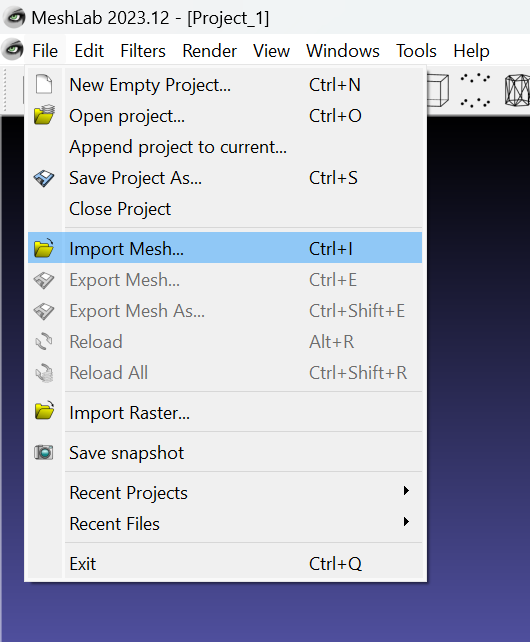
\includegraphics[scale=0.45]{images/importar_01.png}
    \caption{Carga de un archivo de puntos}
\end{figure}

Este es el resultado tras la importación:

\begin{figure}[H]
    \centering
    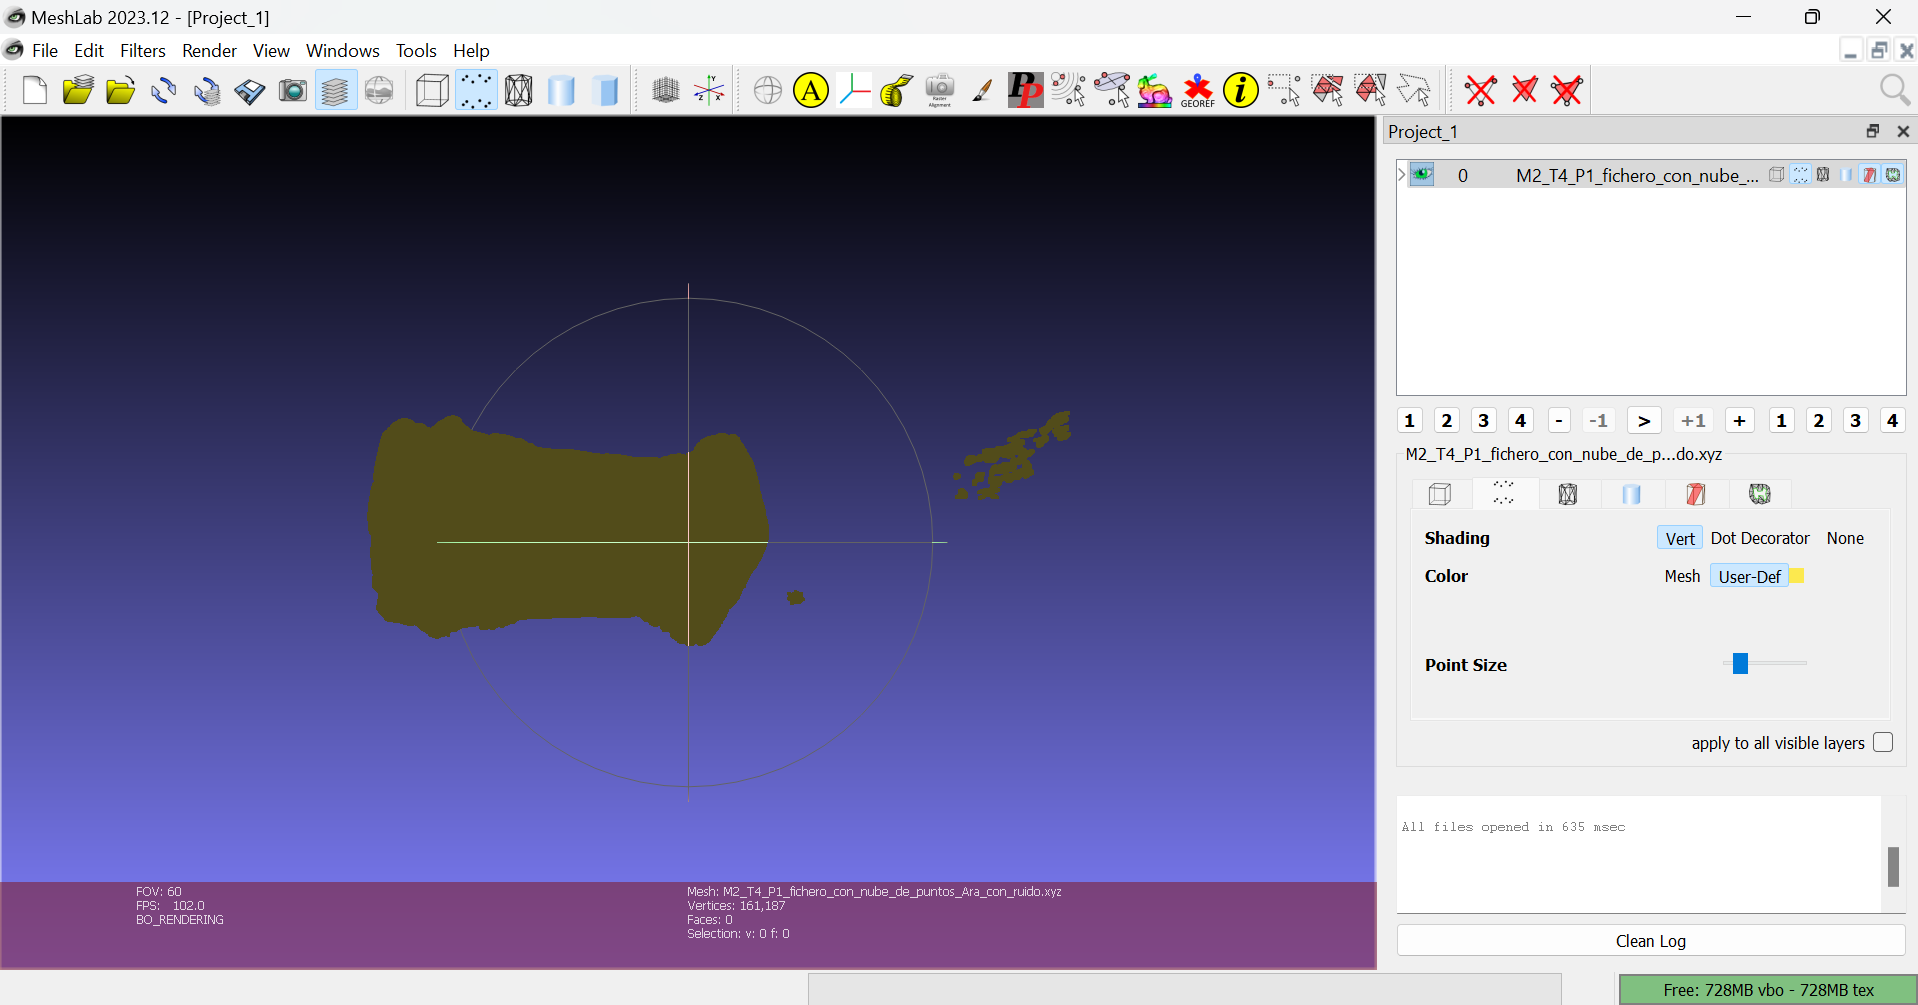
\includegraphics[scale=0.34]{images/importar_02.png}
    \caption{Fichero importado}
\end{figure}

\section{Eliminación del ruido}

Para eliminar el ruido podemos utilizar una herramienta de selección y eliminarlo directamente. Las herramientas de selección y eliminación se encuentran en esta zona del programa:

\begin{figure}[H]
    \centering
    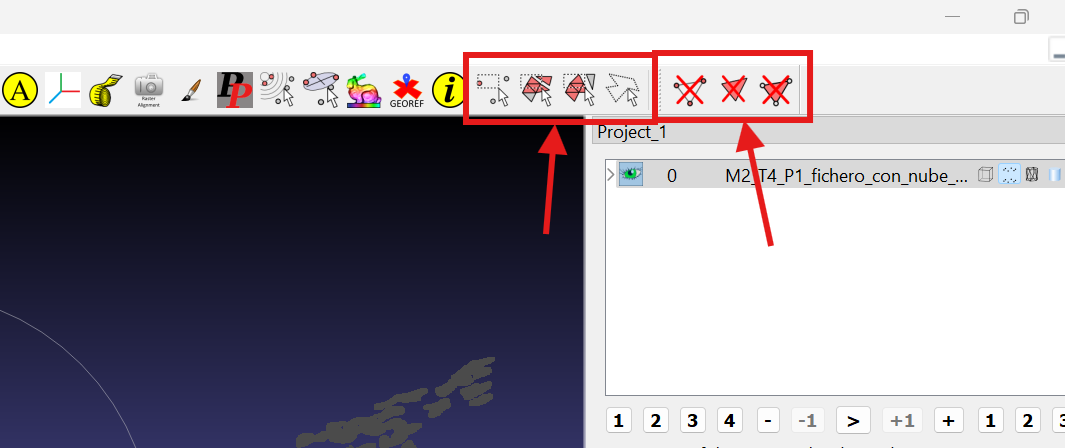
\includegraphics[scale=0.55]{images/ruido_01.png}
    \caption{Selección y borrado}
\end{figure}

\begin{itemize}
    \item El primer rectángulo tiene herramientas de selección
    \item El segundo rectángulo tiene herramientas de borrado
\end{itemize}

\textit{Tip: pasando el puntero por encima te pone qué selecciona y qué borra cada herramienta}

~\\

Para poder trabajar sobre la malla, primero deberemos clonarla. Para ello hacemos \textit{click derecho} sobre ella, y le damos a \textit{``Duplicate current layer''}. Ahora, en nuestro caso, queremos eliminar estas ``nubes'':

\begin{figure}[H]
    \centering
    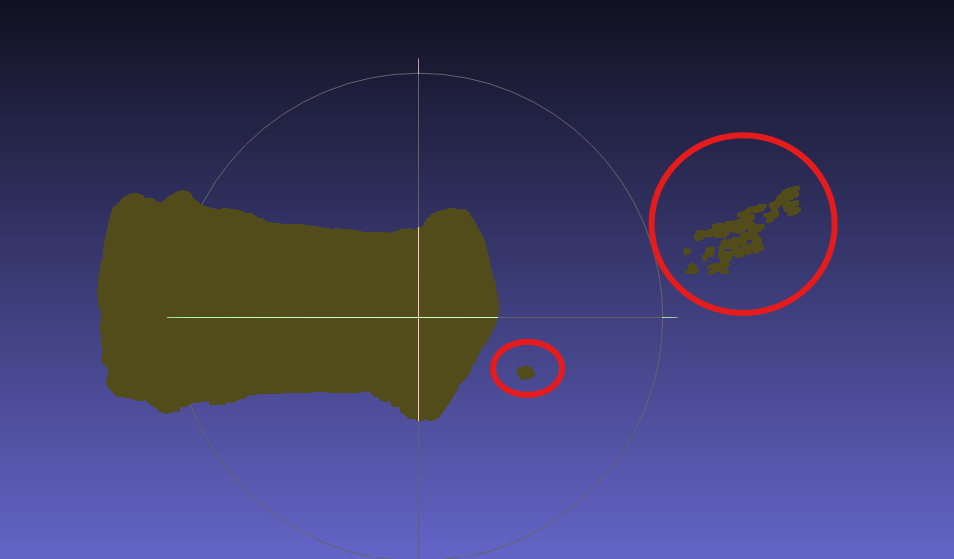
\includegraphics[scale=0.45]{images/ruido_02.png}
    \caption{Ruido que queremos eliminar}
\end{figure}

\pagebreak

Al ser una nube de puntos, deberemos utilizar la \textbf{primera herramienta de selección y borrado} \textit{(select vertices + delete selected vertices)}. El resultado seleccionar y borrar:

\begin{figure}[H]
    \centering
    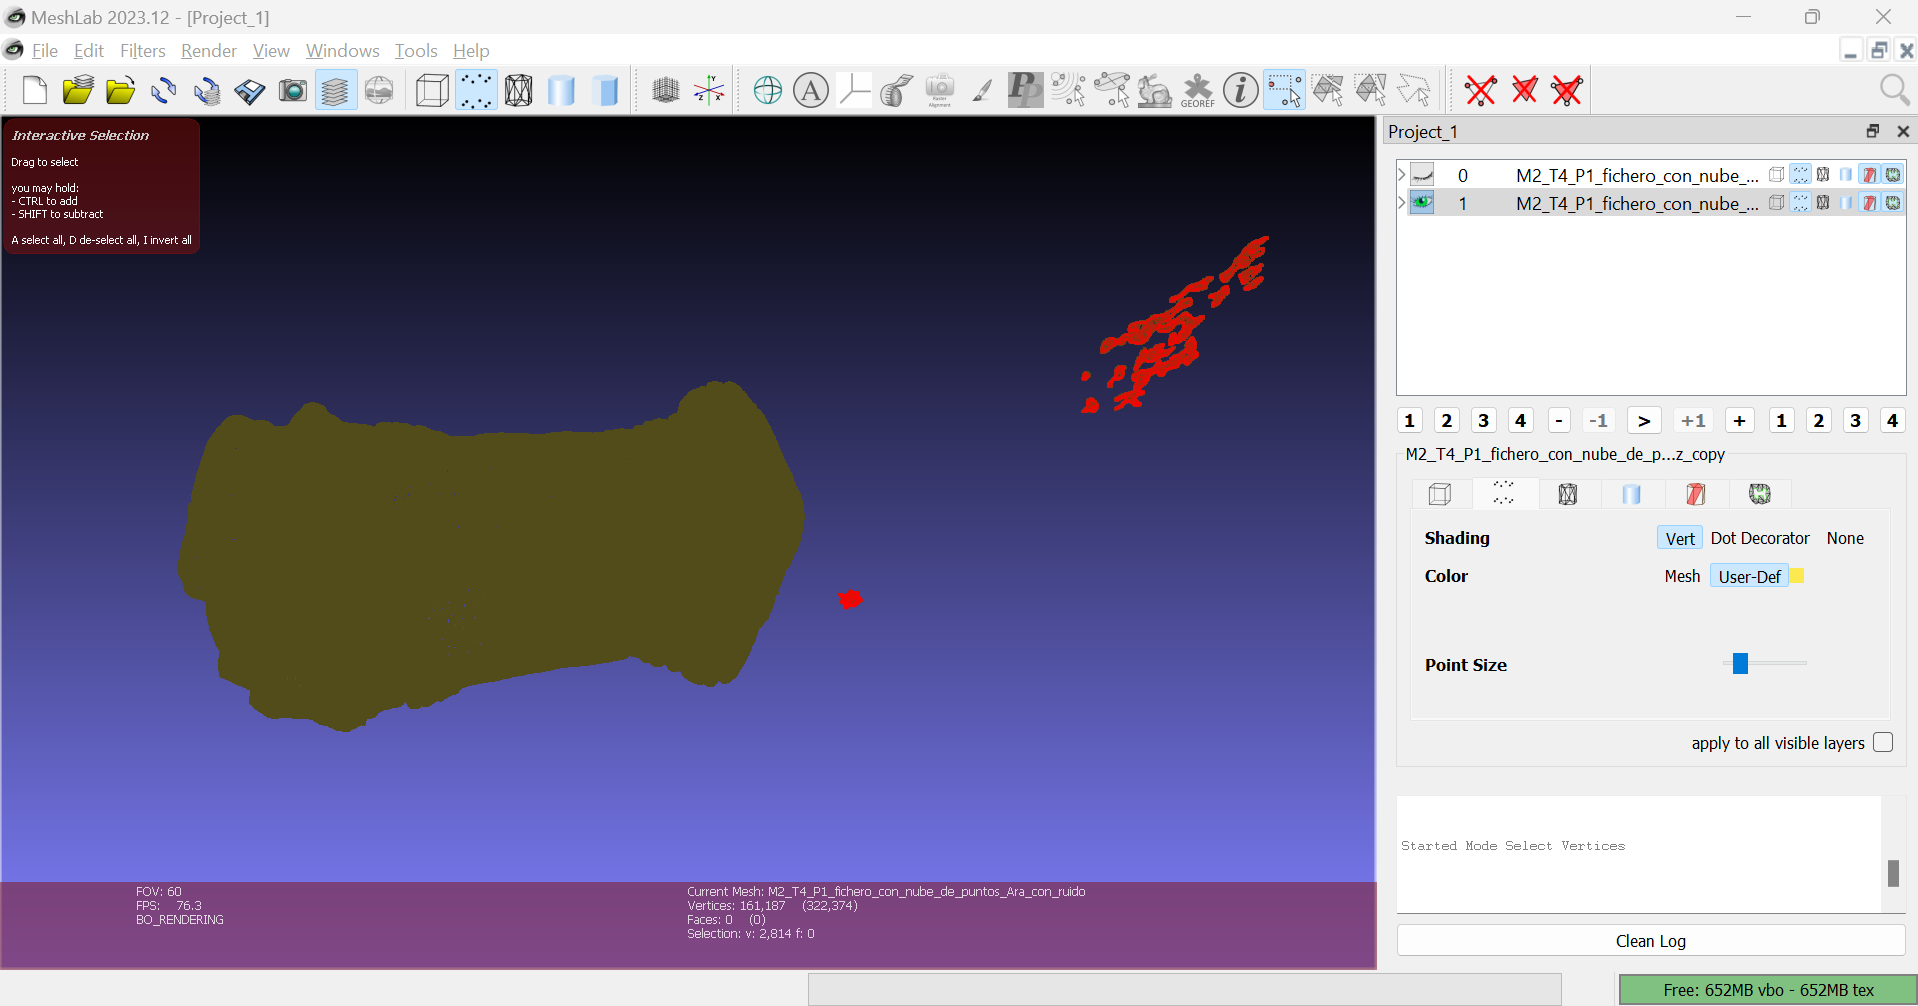
\includegraphics[scale=0.34]{images/ruido_03.png}
    \caption{Ruido seleccionado}
\end{figure}

\begin{figure}[H]
    \centering
    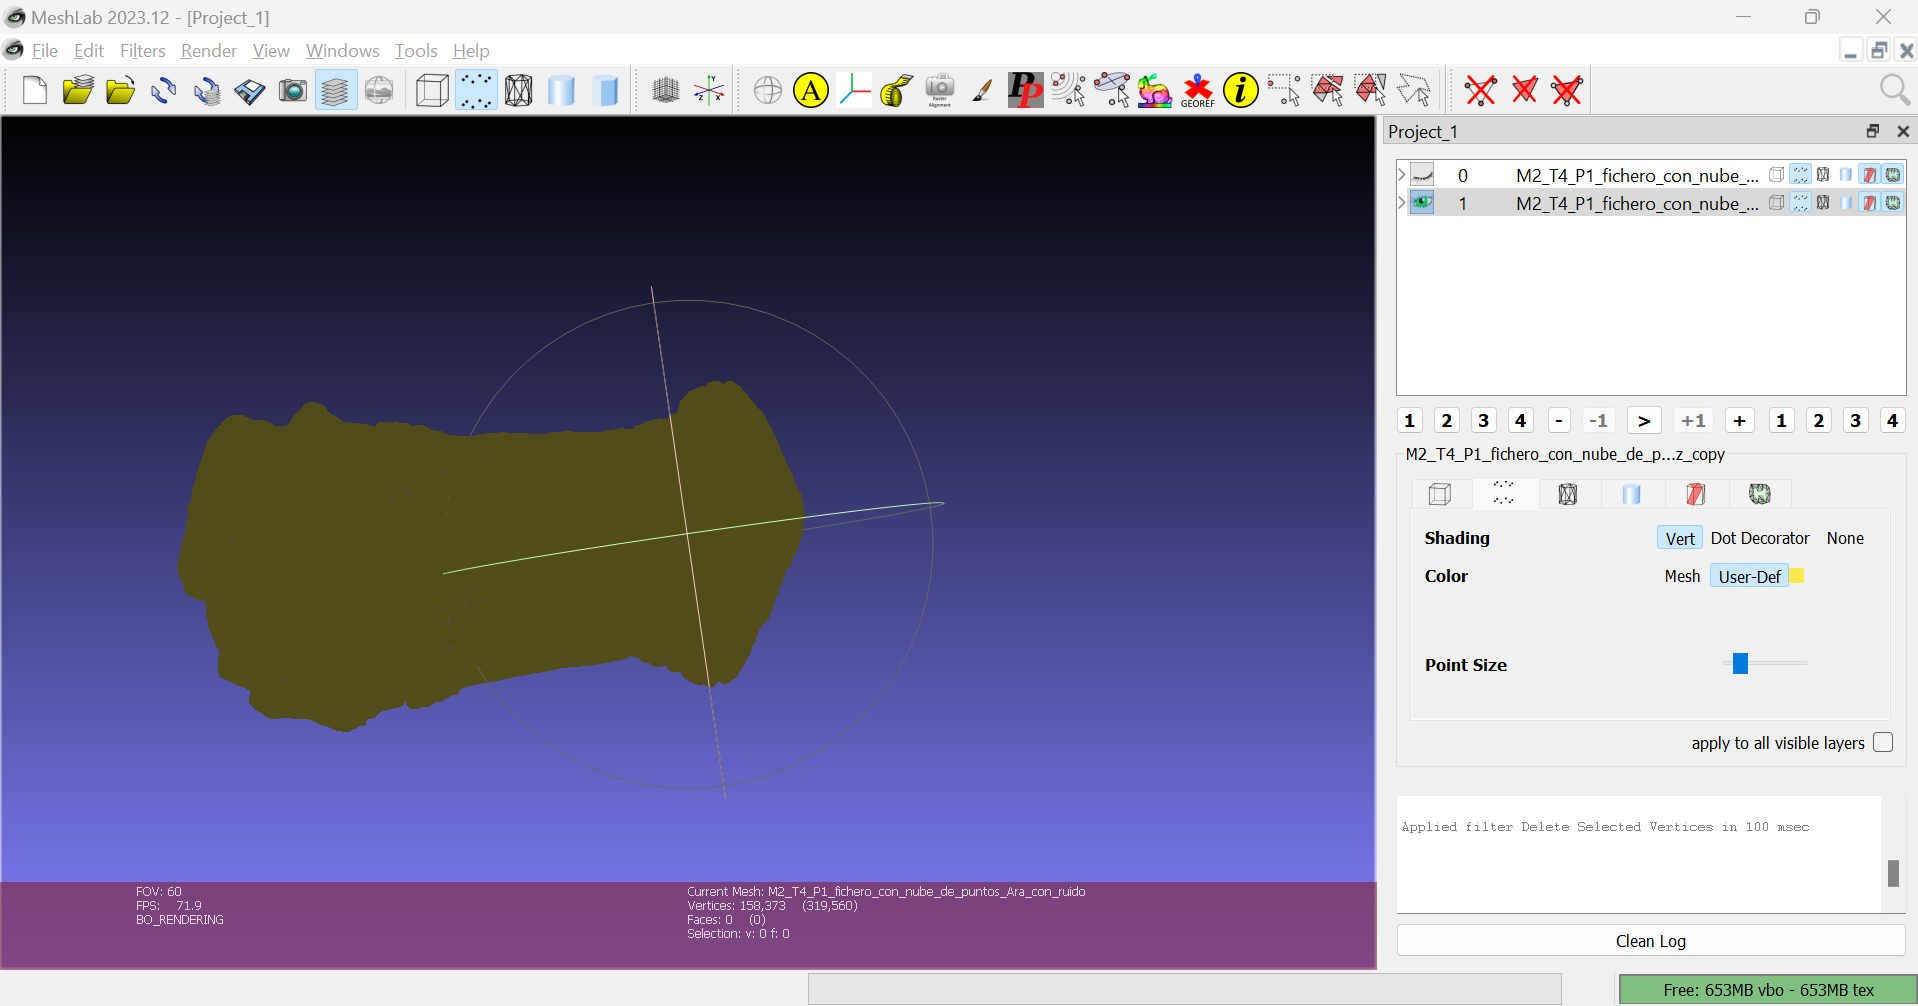
\includegraphics[scale=0.34]{images/ruido_04.png}
    \caption{Ruido borrado}
\end{figure}

\pagebreak

\section{Generación de las normales hacia fuera}

Para calcular las normales de luz de los puntos deberemos hacer click en las siguientes secciones: \textbf{\textit{Filters → Normals, Curvatures and Orientation → Compute normals for pointsets}}:

\begin{figure}[H]
    \centering
    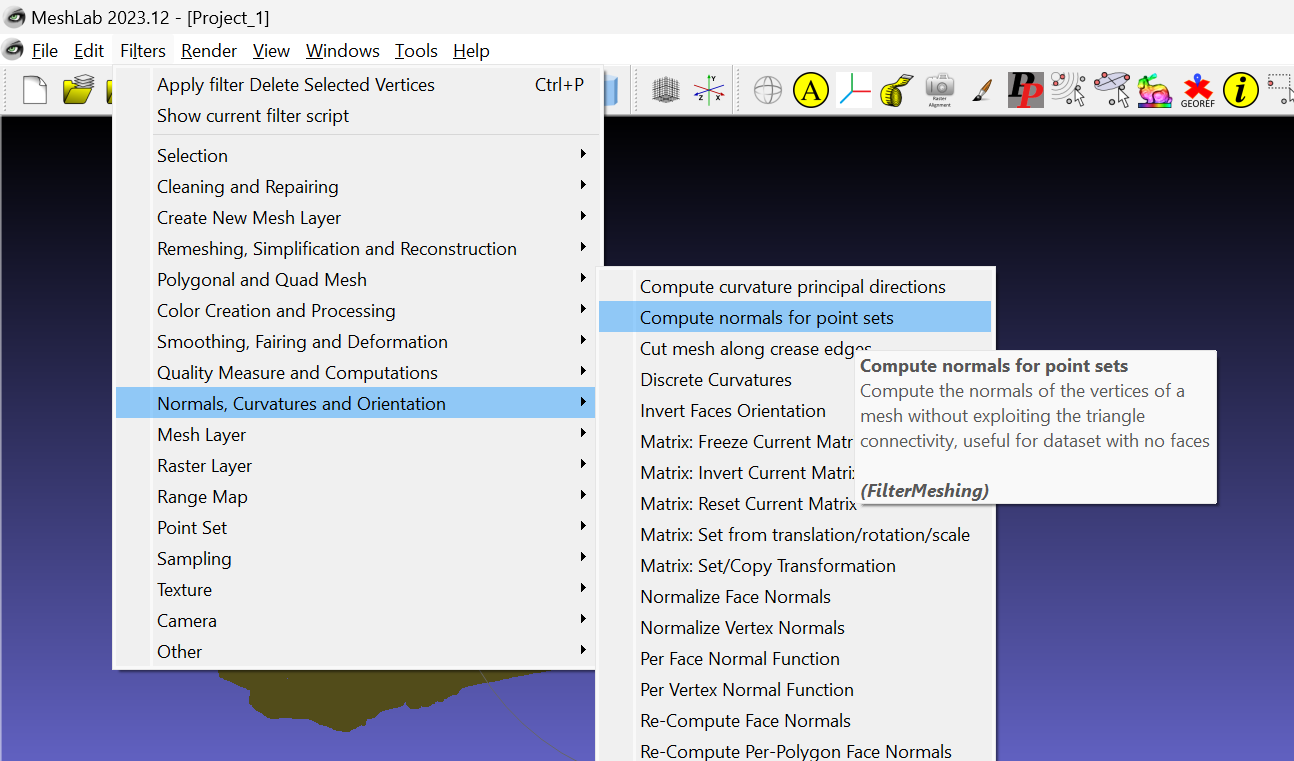
\includegraphics[scale=0.34]{images/normales_01.png}
    \caption{Panel de selección}
\end{figure}

Tras esto se nos desplegará un panel, en el deberemos ir haciendo pruebas con el valor \textit{Neighbour num}. Yo he encontrado que con valor 5 la pieza se ve bastante bien:

\begin{figure}[H]
    \centering
    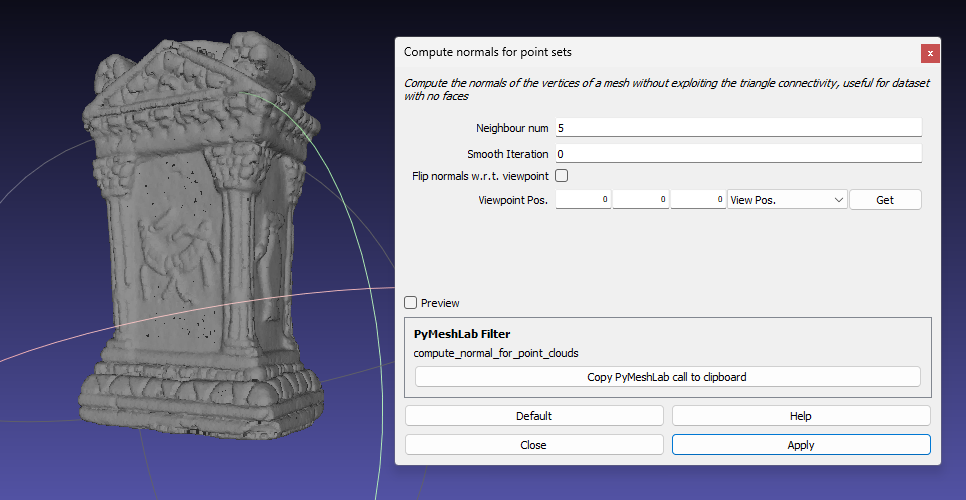
\includegraphics[scale=0.44]{images/normales_02.png}
    \caption{Neighbour num: 5}
\end{figure}

\section{Obtención de la primera malla mediante Poisson}

Para reconstruir mediante Screened Poisson tenemos que seguir la siguiente selección: \textbf{\textit{Filters → Remeshing, Simplification and Reconstruction → Surface Reconstruction: Screened Poisson}}:

\begin{figure}[H]
    \centering
    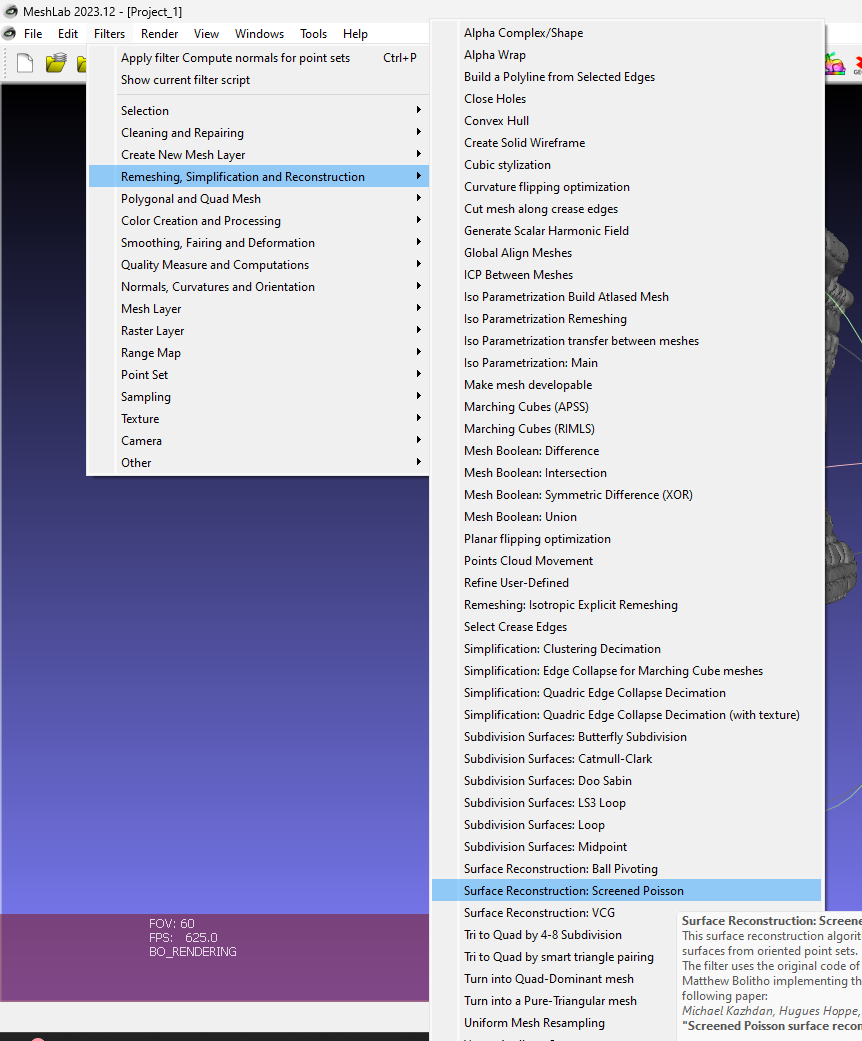
\includegraphics[scale=0.44]{images/poisson_01.png}
    \caption{Panel de selección}
\end{figure}

\pagebreak

Se nos abrirá entonces el siguiente panel y deberemos jugar con el parámetro \textit{Reconstruction depth}, tenemos que intentar no perder número de puntos para no perder calidad, para este caso partimos de 158.373 vértices. Con el valor 8 se nos quedaba un poco corto, así que lo he subido a 9 y nos quedamos con 476.362 vértices y 952.724 caras:

\begin{figure}[H]
    \centering
    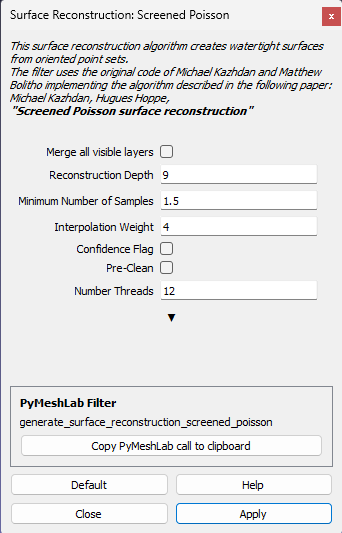
\includegraphics[scale=0.54]{images/poisson_02.png}
    \caption{Panel: Screened Poisson}
\end{figure}

\begin{figure}[H]
    \centering
    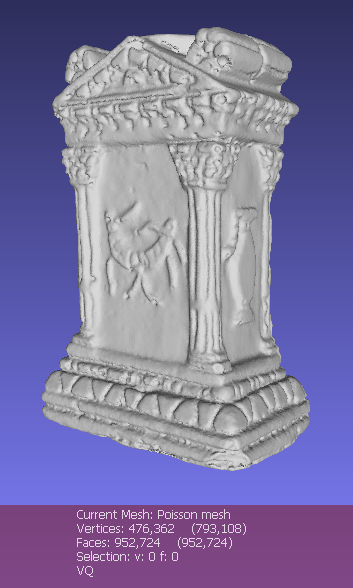
\includegraphics[scale=0.55]{images/poisson_03.png}
    \caption{Resultado de la reconstrucción}
\end{figure}

\pagebreak

\section{Aplicación y explicación de sombras}

Como no tenemos un fichero de textura, vamos a generar sombreado mediante meshlab.

\subsection{Primer sombreado: minnaert.gdp}

Para aplicar este sombreado, nos dirigimos a \textbf{\textit{Render → Shaders → minnaert.gdp}}. Nos aparecerá el siguiente panel con el que podremos probar distintos valores:

\begin{figure}[H]
    \centering
    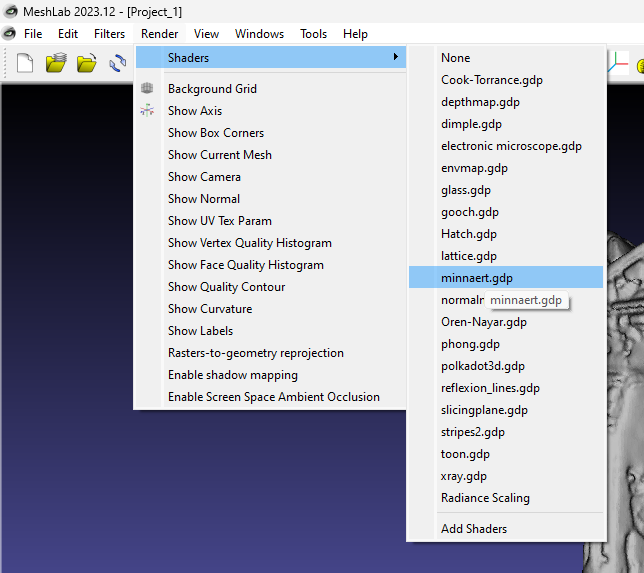
\includegraphics[scale=0.55]{images/sombras_01.png}
    \caption{Panel de selección}
\end{figure}

\begin{figure}[H]
    \centering
    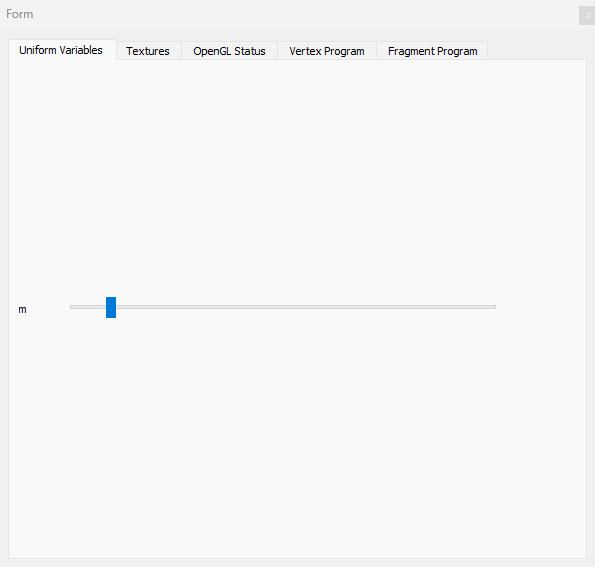
\includegraphics[scale=0.55]{images/sombras_02.png}
    \caption{Panel: minnaert.gdp}
\end{figure}

\begin{figure}[H]
    \centering
    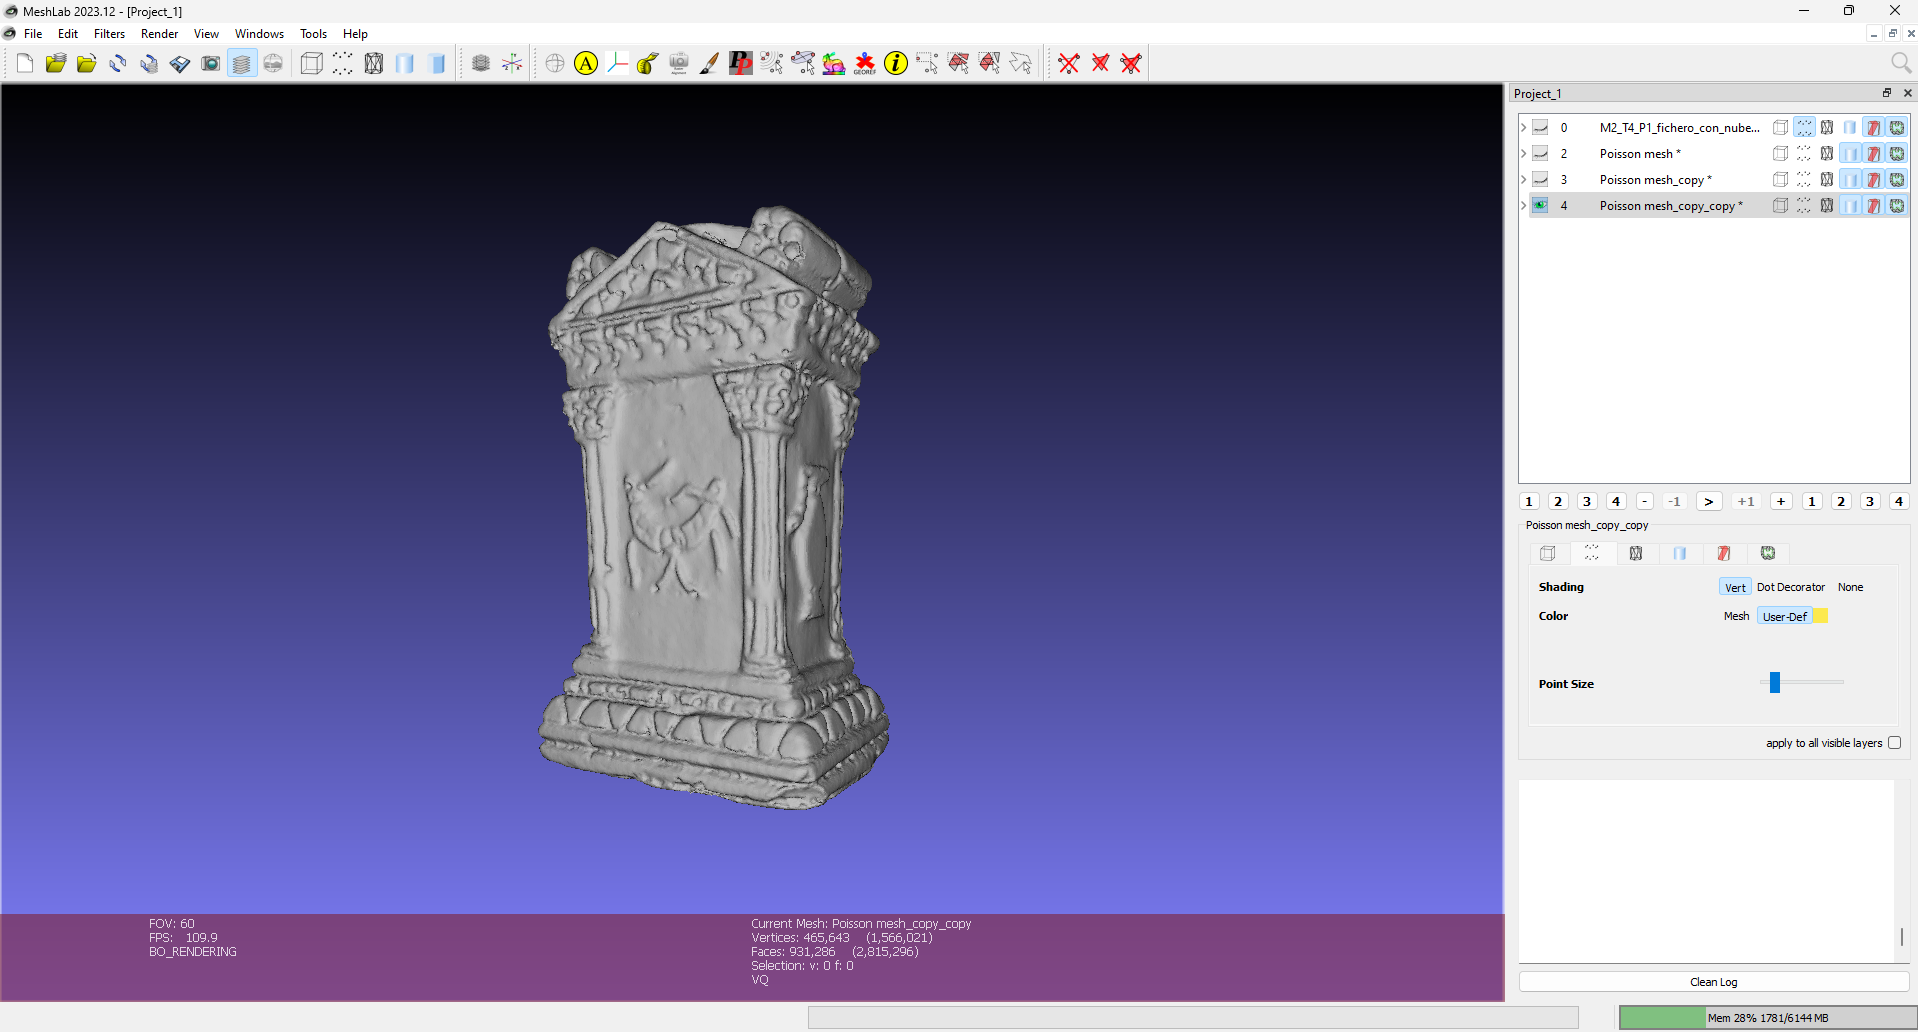
\includegraphics[scale=0.24]{images/sombras_03.png}
    \caption{Resultado del sombreado con minnaert.gdp}
\end{figure}

\pagebreak

\subsection{Segundo sombreado: Cook-Torrance.gdp}

Igual que antes, seleccionamos a \textbf{\textit{Render → Shaders → Cook-Torrance.gdp}} y ajustamos al gusto las varillas:

\begin{figure}[H]
    \centering
    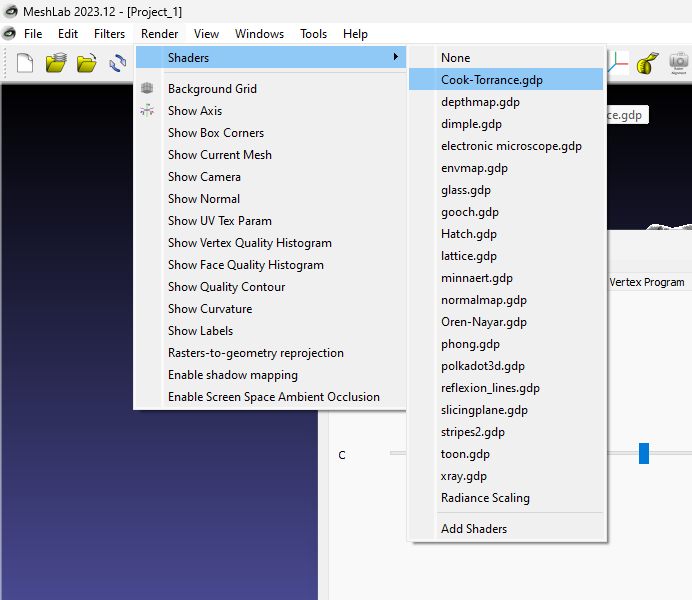
\includegraphics[scale=0.55]{images/sombras_04.png}
    \caption{Panel de selección}
\end{figure}

\begin{figure}[H]
    \centering
    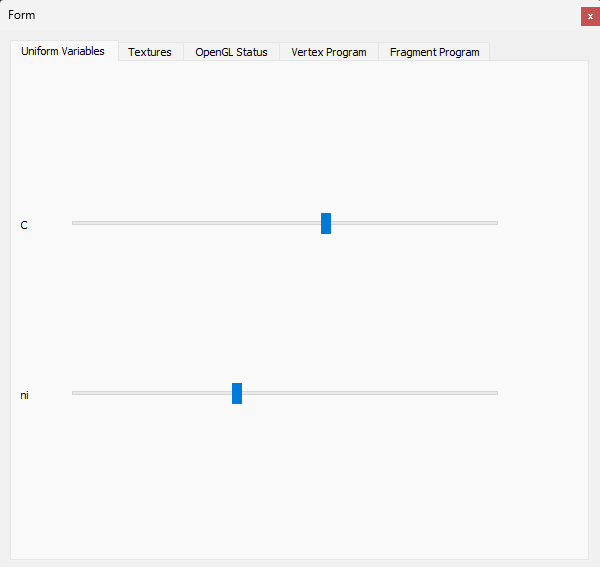
\includegraphics[scale=0.44]{images/sombras_05.png}
    \caption{Panel: Cook-Torrance.gdp}
\end{figure}

\begin{itemize}
    \item \textbf{C}: ilumina u oscurece las caras
    \item \textbf{ni}: ilumina u oscurece las aristas
\end{itemize}

\begin{figure}[H]
    \centering
    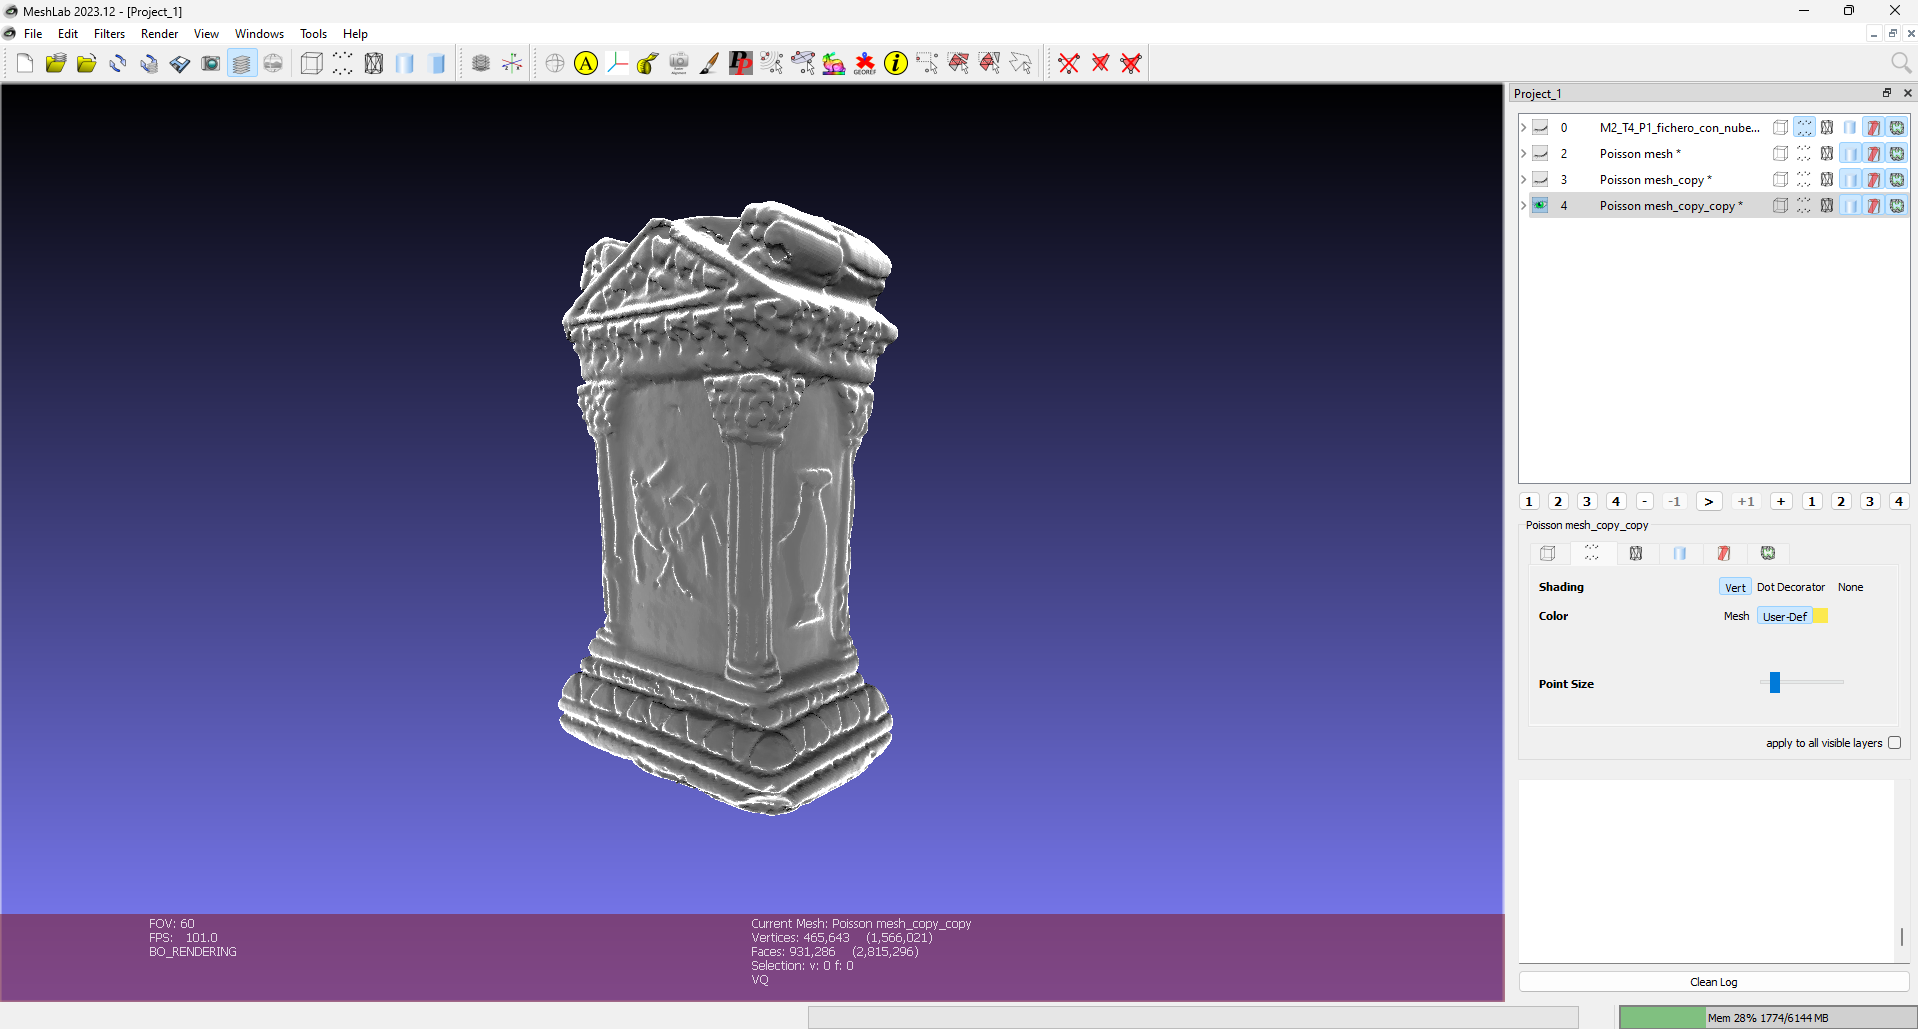
\includegraphics[scale=0.24]{images/sombras_06.png}
    \caption{Resultado del sombreado con Cook-Torrance.gdp}
\end{figure}

\pagebreak

\section{Aplicación y explicación de filtros}

Tras generar una malla, esta puede tener algunas imperfecciones y deberemos limpiarla, para ello podemos servirnos de los distintos filtros que las herramientas ofrezcan.

\subsection{Primer filtro: Remove duplicate vertices}

En este primer filtrado eliminaré los vértices duplicados, para ello iré a las siguientes secciones: \textbf{\textit{Filters → Cleaning and Repairing → Remove duplicate vertices}}. Este es el resultado:

\begin{figure}[H]
    \centering
    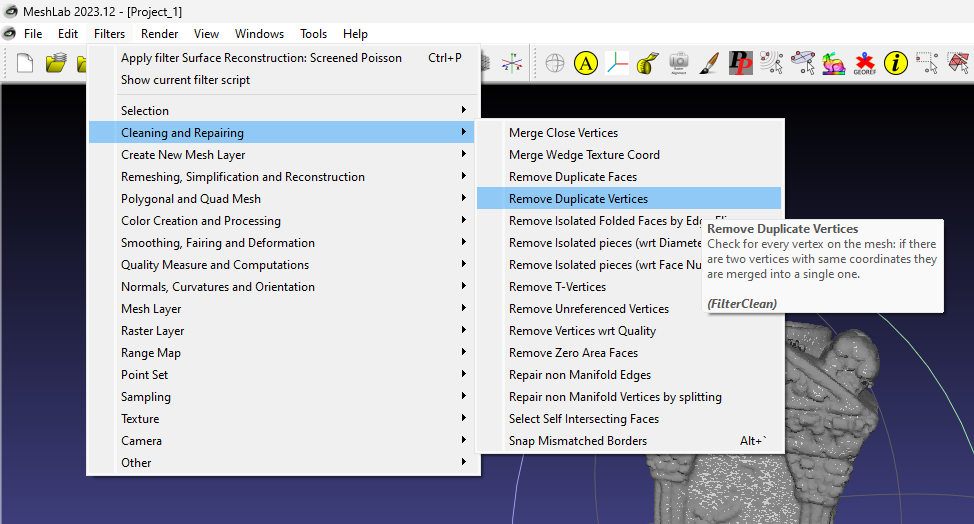
\includegraphics[scale=0.44]{images/filtro_03.png}
    \caption{Panel de selección}
\end{figure}

\begin{figure}[H]
    \centering
    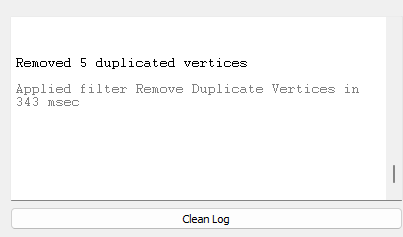
\includegraphics[scale=0.65]{images/filtro_01.png}
    \caption{Resultado en el log}
\end{figure}

Pasamos de 476.362 vértices y 952.724 caras → 476.357 vértices y 952.714 caras

\subsection{Segundo filtro: Remove T-Vertices}

Los T-Vértices son vértices que tocan a una arista. Para limpiar esta \textit{``malformación''} tenemos que ir a \textbf{\textit{Filters → Cleaning and Repairing → Remove T-Vertices}}:

\begin{figure}[H]
    \centering
    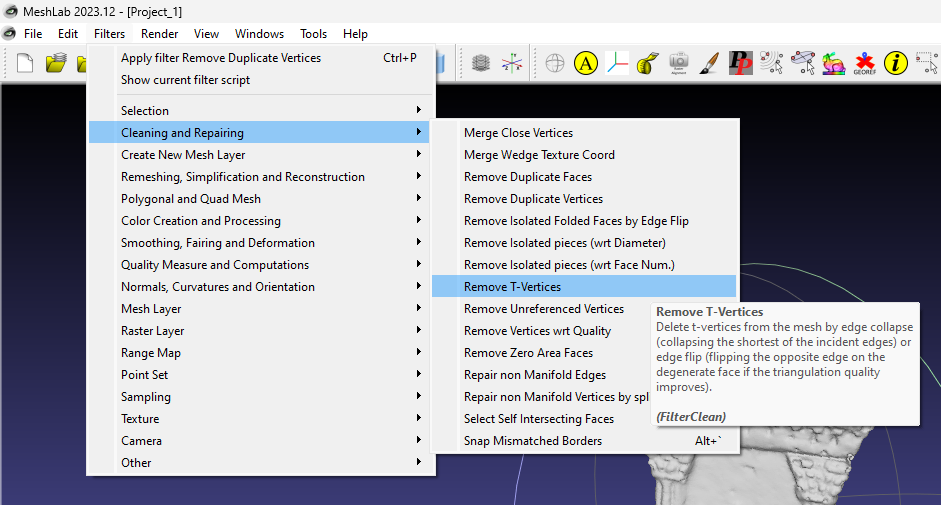
\includegraphics[scale=0.34]{images/filtro_04.png}
    \caption{Panel de selección}
\end{figure}

Se nos despliega el siguiente menú, el método utilizado para eliminarlas será \textit{``Edge Collapse''}:
\begin{figure}[H]
    \centering
    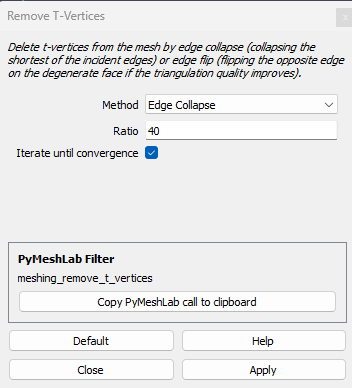
\includegraphics[scale=0.65]{images/filtro_05.png}
    \caption{Panel: Remove T-Vertices}
\end{figure}

\begin{figure}[H]
    \centering
    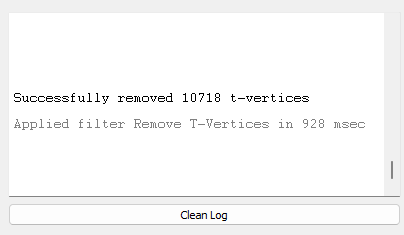
\includegraphics[scale=0.65]{images/filtro_02.png}
    \caption{Resultado en el log}
\end{figure}

Pasamos de 476.357 vértices y 952.714 caras → 465.643 vértices y 931.278 caras.

\pagebreak

\section{Captura de pantalla con Snapshot}

MeshLab ofrece una herramienta para hacer capturas de pantalla. Para utilizarla podemos ir a \textbf{\textit{File → Save snapshot}}:

\begin{figure}[H]
    \centering
    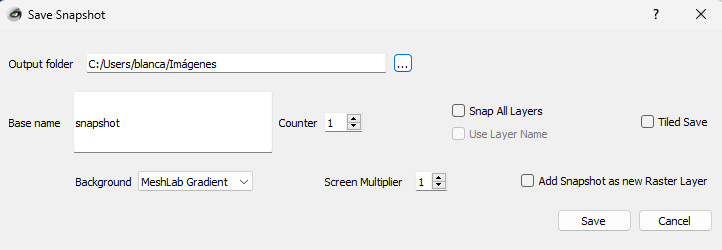
\includegraphics[scale=0.65]{images/snap_01.png}
    \caption{Panel de selección}
\end{figure}

Tras esto se nos desplegará un recuadro en el que tendremos que seleccionar una carpeta en la que guardar el documento, y darle a \textit{``Save''}:

\begin{figure}[H]
    \centering
    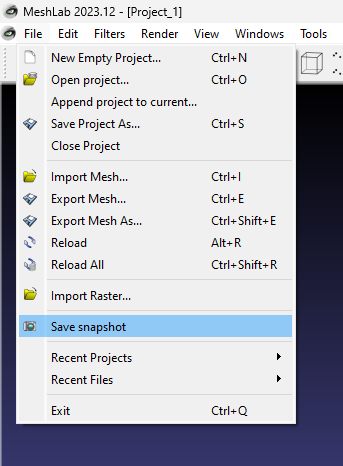
\includegraphics[scale=0.65]{images/snap_02.png}
    \caption{Panel: snapshot}
\end{figure}

\begin{figure}[H]
    \centering
    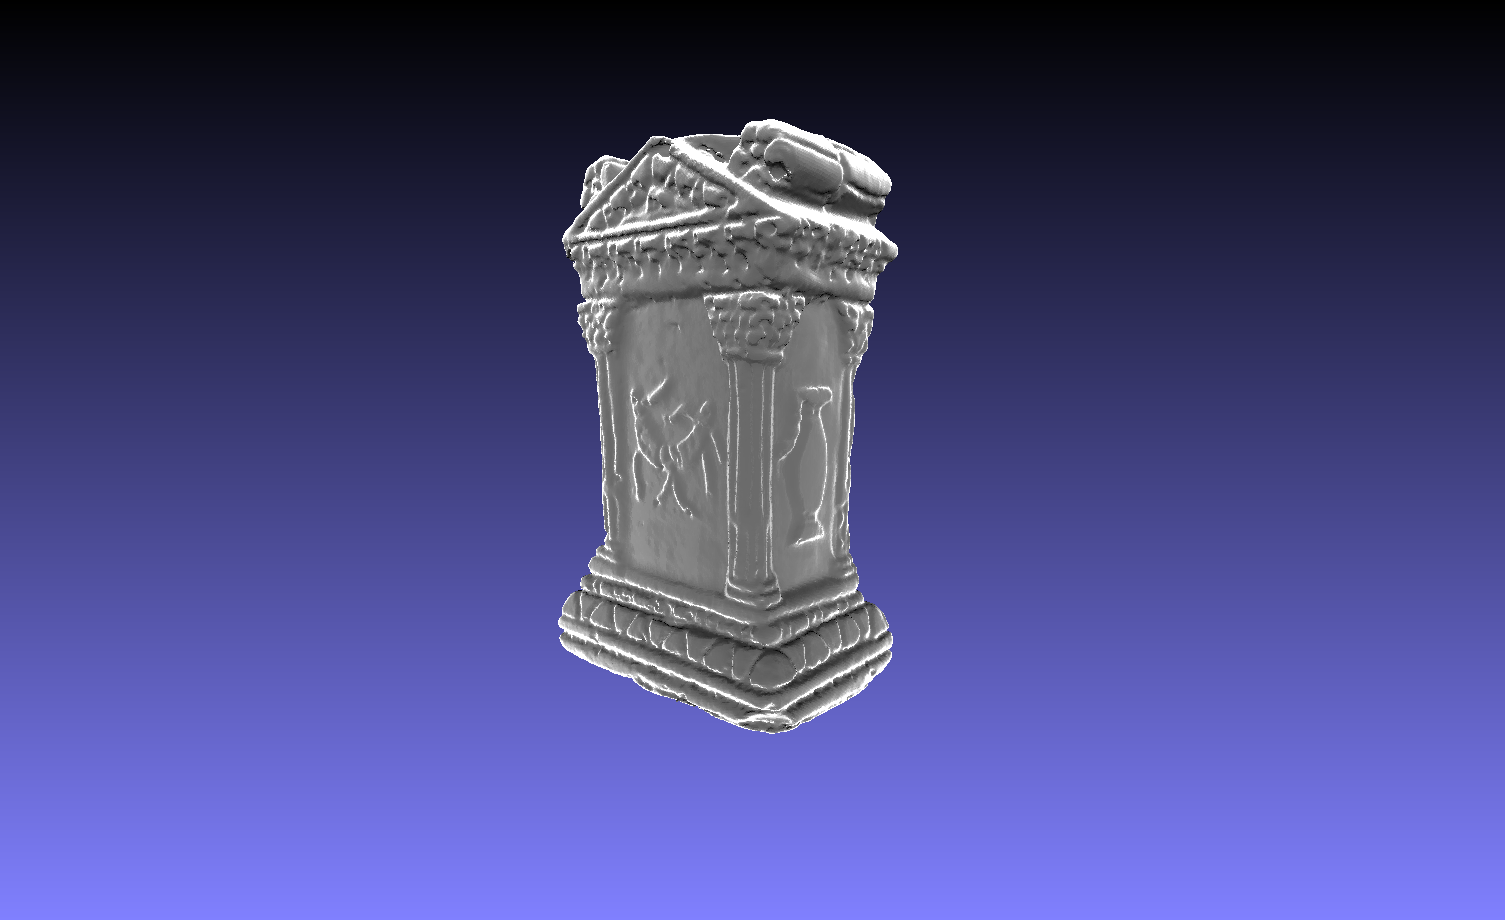
\includegraphics[scale=0.25]{images/snap_03.png}
    \caption{Resultado snapshot}
\end{figure}

\end{document}
